\graphicspath{{../../S21_Volume_du_pave_du_prisme_et_du_cylindre/Images/}}

\themeM
\chapter{Volume du pavé, du prisme et du cylindre}
\label{S21}

\programme%
   {\item Volume d'un prisme, d'un cylindre.
    \item Correspondance entre volume et contenance : $\Capa{1} =\Vol[dm]{1}$ et $\Capa{1000} =\Vol[m]{1}$.}
   {\item Vérifier le cohérence des résultats au niveau des unités.
    \item Effectuer des conversions d'unités de volumes.}

\vfill

\begin{debat}{Débat : $\Capa{1} =\Vol[dm]{1}$}
   Cette correspondance est à connaître. Pourtant, elle ne paraît pas si naturelle que cela : elle signifie que l'eau contenue dans une bouteille d'un litre remplirait exactement un cube de \Lg[dm]{1} de côté.
   \tcblower
      {\psset{unit=0.9}
      \begin{pspicture}(0,0)(6,5.5)
         \psline(0.5,0.5)(0.5,3.75) %bouteille
         \psline(2,0.5)(2,3.75)
         \psarc(1.5,3.75){0.5}{0}{90}
         \psarc(1,3.75){0.5}{90}{180}
         \psline(1,4.25)(1,5)
         \psline(1.5,4.25)(1.5,5)
         \psellipticarc(1.25,0.5)(0.75,0.3){180}{0}
         \psellipticarc(1.25,3.5)(0.75,0.3){180}{0}
         \psellipticarc[linestyle=dashed](1.25,3.5)(0.75,0.3){0}{180}
         \psellipse(1.25,5)(0.25,0.1)
         \rput(1.25,2){\Capa{1}}
         \psframe(3,0.5)(5,2.5) %cube
         \psline(3,2.5)(3.75,3.25)(5.75,3.25)(5.75,1.25)(5,0.5)
         \psline(5,2.5)(5.75,3.25)
         \rput(4,0.2){$\Vol[dm]{1} =\Lg{10}$}
         \rput(4,1.5){$\Vol[dm]{1}$}
      \end{pspicture}}
\end{debat}

\hfill {\gray Vidéo : \href{https://www.youtube.com/watch?v=kNicKj-PIB4&t=174s}{\bf Les volumes}, chaîne {\it Rapémathiques} d'A'Rieka.}


%%% Approche %%%
\begin{Maquette}[Cours]{Theme={Activité d'approche},Couleur={SteelBlue}}

   \AAtitre{Séquence 21 : Des pavés cachés}
   
      {\it Objectifs : calculer le volume d'un pavé droit, d'un assemblage de solides ; résoudre un problème dans le domaine des grandeurs et mesures.} Matériel à disposition : des cubes à emboîter, des briques types kapla ou Lego, des boites, des morceaux de sucres.
      
      \begin{AActivite}

         \begin{minipage}{11.5cm}
            \AApartie{On me voit assez bien !} \par
            Ma petite s\oe ur empile des cubes les uns sur les autres, tous de même forme. Voici sa construction. \par
            Combien a-t-elle empilé de cubes ?
            \vspace*{1.7cm}
         \end{minipage}
         \qquad
         \begin{minipage}{4.5cm}
            \VueCubes[Creation,Largeur=5,Profondeur=5,Hauteur=5,Angle=60,Seul,CouleurCube=1.5SteelBlue]{3,4,5,5,5,2,4,4,5,5,1,3,4,4,5,1,2,3,4,4,1,1,1,2,3}
         \end{minipage}
         
         \bigskip

         \begin{minipage}{9cm}
            \AApartie{On me voit un peu moins !}
            Mon grand-père veut construire la même jardinière que sur la photo ci-contre. \par
            De combien de briques aura-t-il besoin ?
            \vspace*{2.2cm}
         \end{minipage}
         \qquad
         \begin{minipage}{7cm}
            \includegraphics[width=6.5cm]{jardiniere}
         \end{minipage}
         
         \bigskip

         \AApartie{On ne me voit plpas du tout !}
            L’entreprise Sucromania fabrique du sucre en morceaux. Elle souhaite conditionner ses morceaux dans un emballage parallélépipédique de \Lg[mm]{280} de long, \Lg[mm]{140} de large et \Lg[mm]{70} de hauteur. \par
            Sachant qu’un sucre a la forme d’un pavé droit de \Lg[mm]{14} de long, \Lg[mm]{14} de large et \Lg[mm]{10} de hauteur, combien de sucres peut-elle mettre au maximum afin d’optimiser son emballage ?
            \vspace*{7cm}

      \end{AActivite}

      \vfill\hfill{\it\footnotesize Source : d'après \href{https://eduscol.education.fr/document/13132/download}{\og La résolution de problèmes mathématiques au collège}, MENJS, p.136}

\end{Maquette}


%%%Trace écrite %%%
\begin{Maquette}[Cours]{Theme={Trace écrite},Couleur={0.4[SteelBlue,Black]}}

   %%%1
   \section{Volume par dénombrement}

      \begin{definition*}{}
         Le \textbf{volume} est une grandeur physique qui mesure l'espace occupé par celui-ci.
      \end{definition*}

      \begin{exemple*}{}
         {\psset{unit=0.6}
         Ces trois objets n'ont pas la même forme mais occupent la même quantité d'espace, ils ont donc le même volume.
         \begin{center}
            \begin{pspicture}(0,-1)(13,3.5)
               \psset{linecolor=DodgerBlue}
               \psframe(0,0)(3,2)
               \psline(1,0)(1,2)(1.5,2.5)
               \psline(2,0)(2,2)(2.5,2.5)
               \psline(0,1)(3,1)(3.5,1.5)
               \psline(3,0)(3.5,0.5)(3.5,2.5)(0.5,2.5)(0,2)
               \psline(3,2)(3.5,2.5)
               \psset{linecolor=Crimson}
               \pspolygon(5,0)(9,0)(9,2)(8,2)(8,1)(6,1)(6,2)(5,2)
               \psline(5,1)(6,1)(6,0)
               \psline(7,0)(7,1)(7.5,1.5)
               \psline(9,0)(9.5,0.5)(9.5,2.5)(8.5,2.5)(8,2)
               \psline(9,2)(9.5,2.5)
               \psline(9.5,1.5)(9,1)(8,1)(8,0)
               \psline(5,2)(5.5,2.5)(6.5,2.5)(6.5,1.5)(8,1.5)
               \psline(6,2)(6.5,2.5)
               \psline(6,1)(6.5,1.5)    
               \psset{linecolor=ForestGreen}  
               \pspolygon(11,0)(14,0)(14,1)(13,1)(13,2)(12,2)(12,3)(11,3)
               \psline(12,0)(12,1)(11,1)
               \psline(13,0)(13,1)(12,1)(12,2)(11,2)
               \psline(14,0)(14.5,0.5)(14.5,1.5)(13.5,1.5)(13.5,2.5)(12.5,2.5)(12.5,3.5)(11.5,3.5)(11,3)
               \psline(14,1)(14.5,1.5)
               \psline(13,2)(13.5,2.5)
               \psline(12,3)(12.5,3.5)
               \psline(13,1)(13.5,1.5)
               \psline(12,2)(12.5,2.5)
            \end{pspicture}
         \end{center}
         Si l'unité de volume est un cube \psline(0,1)(0,0)(1,0)(1,1)(0,1)(0.5,1.5)(1.5,1.5)(1.5,0.5)(1,0) \psline(1,1)(1.5,1.5) \hskip1cm le volume de ces trois solides est de 6 unités de volume.}
      \end{exemple*}

      Il existe deux unités en dimension 3 : les unités de volumes en \og cube \fg{} et les unités de capacité en \og litre \fg. 

      \begin{definition*}{}
         \begin{itemize}
            \item Lorsque l'unité de volume est un cube de \Lg[m]{1} d'arête, cela représente \Vol[m]{1}.
            \item Le {\bf litre} (L) est une unité de capacité valant \Vol[dm]{1}. On a alors $\Capa{1} =\Vol[dm]{1}$ et $\Capa{1000} =\Vol[m]{1}$.
         \end{itemize}
      \end{definition*}

      Pour effectuer un changement d'unité de volume, on reprend les mêmes préfixes que pour les changements de longueur, et on impose pour chacun d'eux trois colonnes au tableau. \medskip

      \Tableau[Cube,Capacite,FlechesH]{39621/12}

      \begin{exemple*}{}
         \Vol[dam]{0,0039621} = \Vol[m]{3,9621} = \Vol[dm]{3962,1} = \Capa{3962,1} = \Vol[cm]{3962100}.
      \end{exemple*}
         
   
   %%%2
   \section{Volumes classiques}

      \begin{minipage}[t]{5.5cm}
         \Formule[Volume,Solide=pave,Largeur=5.5cm,Ancre={(2.75,-2)},Couleur=yellow!10]
      \end{minipage}
      \qquad
      \begin{minipage}[t]{4.5cm}
         \Formule[Volume,Solide=prisme,Largeur=4.5cm,Ancre={(2.25,-2)},Couleur=yellow!10]
      \end{minipage}
      \qquad
      \begin{minipage}[t]{6cm}
         \Formule[Volume,Solide=cylindre,Largeur=6cm,Ancre={(3,-2)},Couleur=yellow!10]
      \end{minipage}

\end{Maquette}


%%% Exercices %%%
\begin{Maquette}[Fiche,CorrigeFin,Colonnes=2]{}

   \begin{multicols}{2}

         \begin{exercice}[SLF] %1
            Donner le volume de chaque solide en unités de volume (les volumes sont supposés pleins). \par \bigskip
            \begin{minipage}{1.8cm}
               \VueCubes[Largeur=1,Profondeur=1,Hauteur=1,Angle=30,Seul]{} \par
               {\footnotesize unité de} \par
               {\footnotesize volume} \par \bigskip
               3 \VueCubes[Creation,Largeur=3,Profondeur=2,Hauteur=4,Angle=30,Seul]{0,3,2,4,3,4}
            \end{minipage}
            \begin{minipage}{3.7cm}
               1 \VueCubes[Creation,Largeur=5,Profondeur=4,Hauteur=3,Angle=-30,Seul]{3,3,3,3,3,3,3,3,3,3,3,3,3,3,3,3,3,3,3,3,3,3,3,3} \par \bigskip
               4 \VueCubes[Creation,Largeur=5,Profondeur=5,Hauteur=3,Angle=-30,Seul]{1,1,1,1,1,1,2,2,2,1,1,2,3,2,1,1,2,2,2,1,1,1,1,1,1}
            \end{minipage}
            \begin{minipage}{2.2cm}
               2 \VueCubes[Creation,Largeur=3,Profondeur=3,Hauteur=3,Angle=30,Seul]{3,3,3,2,2,3,1,2,3} \par \bigskip
               5 \VueCubes[Creation,Largeur=3,Profondeur=3,Hauteur=4,Angle=30,Seul]{1,2,3,2,2,2,2,3,1}
            \end{minipage}
         \end{exercice}
         
         \begin{Solution}
           On note $u$ l'unité de volume.
           \begin{enumerate}
              \item $5\times4\times3 =60$. Donc, \cor{$\mathcal{v}_1 = 60\,u$}.
              \item $3^{3}-(4+1) =27-5 =22$. Donc, \cor{$\mathcal{v}_2 = 22\,u$}.
              \item $7+6+3 =16$. Donc, \cor{$\mathcal{v}_3 = 16\,u$}.
              \item $5^{3}+3^{3}+1 =25+9+1 =$. Donc, \cor{$\mathcal{v}_4 = 35\,u$}.
              \item $6+6+6 =18$. Donc, \cor{$\mathcal{v}_5 = 18\,u$}.
           \end{enumerate}
         \end{Solution}
         
         
         \begin{exercice} %2
            Classer ces pavés du plus petit au plus grand volume.
            \begin{center}
               {\psset{unit=0.5,fillstyle=solid,fillcolor=lightgray}
               \footnotesize
               \begin{pspicture}(1,0.5)(11,9)
                  \pspolygon(1,1)(5,1)(6,2)(6,3.5)(2,3.55)(1,2.5)
                  \psline(1,2.5)(5,2.5)(6,3.5)
                  \psline(5,2.5)(5,1)
                  \rput(3,0.6){\Lg{4}}
                  \rput{90}(0.6,1.75){\Lg{1,5}}
                  \rput{45}(5.8,1.2){\Lg{2,5}}
                  \rput(3.5,3){C}
                  \pspolygon(1,5)(3.5,5)(4.5,6)(4.5,8.5)(2,8.5)(1,7.5)
                  \psline(1,7.5)(3.5,7.5)(4.5,8.5)
                  \psline(3.5,7.5)(3.5,5)
                  \rput(2.25,4.6){\Lg{2,5}}
                  \rput(2.25,6.25){cube}
                  \rput(2.5,8){A}
                  \pspolygon(9,1)(10,1)(10.9,1.9)(10.9,8.9)(9.9,8.9)(9,8)
                  \psline(10,1)(10,8)(10.9,8.9)
                  \psline(10,8)(9,8)
                  \rput(9.4,0.6){\Lg{1}}
                  \rput{45}(10.9,1.15){\Lg{2,2}}
                  \rput{90}(8.6,4.5){\Lg{7}}
                  \rput(10,8.5){B}
               \end{pspicture}}
            \end{center}
         \end{exercice}
         
         \begin{Solution}
            \begin{enumerate}
               \item[A] Le volume du cube A vaut $c^3$ : \par
                  $\mathcal{v}_{\text A} =\Lg{2,5}\times\Lg{2,5}\times\Lg{2,5} =\cor{\Vol[cm]{15,625}}$.
               \item[B] Le volume du pavé haut B vaut $L\times\ell\times h$ : \par
                  $\mathcal{v}_{\text B} =\Lg{2,2}\times\Lg{1}\times\Lg{7} =\cor{\Vol[cm]{15,4}}$.
               \item[C] Le volume du dernier pavé C vaut $L\times\ell\times h$ : \par
                  $\mathcal{v}_{\text C} =\Lg{4}\times\Lg{2,5}\times\Lg{1,5} =\cor{\Vol[cm]{15}}$.
            \end{enumerate}
            On a donc \cor{C < B < A}.
         \end{Solution}
         
         
         \begin{exercice}[SLF] %3
            Associer à chaque mesure l'objet qui lui correspond. \par  
            \Relie[LargeurG=19mm,Ecart=7mm,LargeurD=32mm,Stretch=1.1]
               {\Capa{16}/Maison/2,
               \Vol[hm]{1}/Cartable/6,
               \Vol[mm]{10}/Baignoire/7,
               \Vol[m]{600}/Mer Méditerranée/6,
               \Vol[km]{3700000}/Bille/4,
               \Vol[cm]{1}/Empire State Building/5,
               \Capa{160}/Grain de riz/3}
         \end{exercice}
         
         \begin{Solution}
            \Relie[Solution,Couleur=RoyalBlue,LargeurG=18mm,Ecart=8mm,LargeurD=32mm,Stretch=1.1]
               {\Capa{16}/Maison/2,
               \Vol[hm]{1}/Cartable/6,
               \Vol[mm]{10}/Baignoire/7,
               \Vol[m]{600}/Mer Méditerranée/1,
               \Vol[km]{3700000}/Bille/4,
               \Vol[cm]{1}/Empire State Building/5,
               \Capa{160}/Grain de riz/3}
         \end{Solution}
            
         
         \begin{exercice} %4
            Effectuer les conversions de volumes et capacités :
            \begin{enumerate}
               \item \Vol[dm]{1} = \pointilles \; \Vol[mm]{} \smallskip
               \item \Vol[mm]{200} = \pointilles \; \Vol[cm]{} \smallskip
               \item \Vol[km]{1542} = \pointilles \; \Vol[dam]{} \smallskip
               \item \Capa{1} = \pointilles \; \Capa[dl]{} \smallskip
               \item \Capa[daL]{1,53} = \pointilles \; \Capa[cL]{} \smallskip
               \item \Capa[hL]{1} = \pointilles \; \Vol[cm]{} \smallskip
               \item \Capa{131,2} = \pointilles \; \Vol[m]{} \smallskip
               \item \Vol[cm]{35,635} = \pointilles \; \Capa[dl]{} \smallskip
            \end{enumerate}
         \end{exercice}
         
         \begin{Solution}
            \begin{enumerate}
               \item \Vol[dm]{1} = \cor{\Vol[mm]{1000000}}
               \item \Vol[mm]{200} = \cor{\Vol[cm]{0,2}}
               \item \Vol[km]{1542} = \cor{\Vol[dam]{1542000000}}
               \item \Capa{1} = \cor{\Capa[dL]{10}}
               \item \Capa[daL]{1,53} = \cor{\Capa[cL]{1530}}
               \item \Capa[hL]{1} = \cor{\Vol[cm]{100000}}
               \item \Capa{131,2} = \cor{\Vol[m]{0,1312}}
               \item \Vol[cm]{35,635} = \cor{\Capa[dL]{0,35635}}
            \end{enumerate}
         \end{Solution}
         
         
         \begin{exercice} %5
            Dans chacune des figures suivantes, colorier une base en jaune, repasser une hauteur en rouge puis calculer le volume.
            \begin{center}
               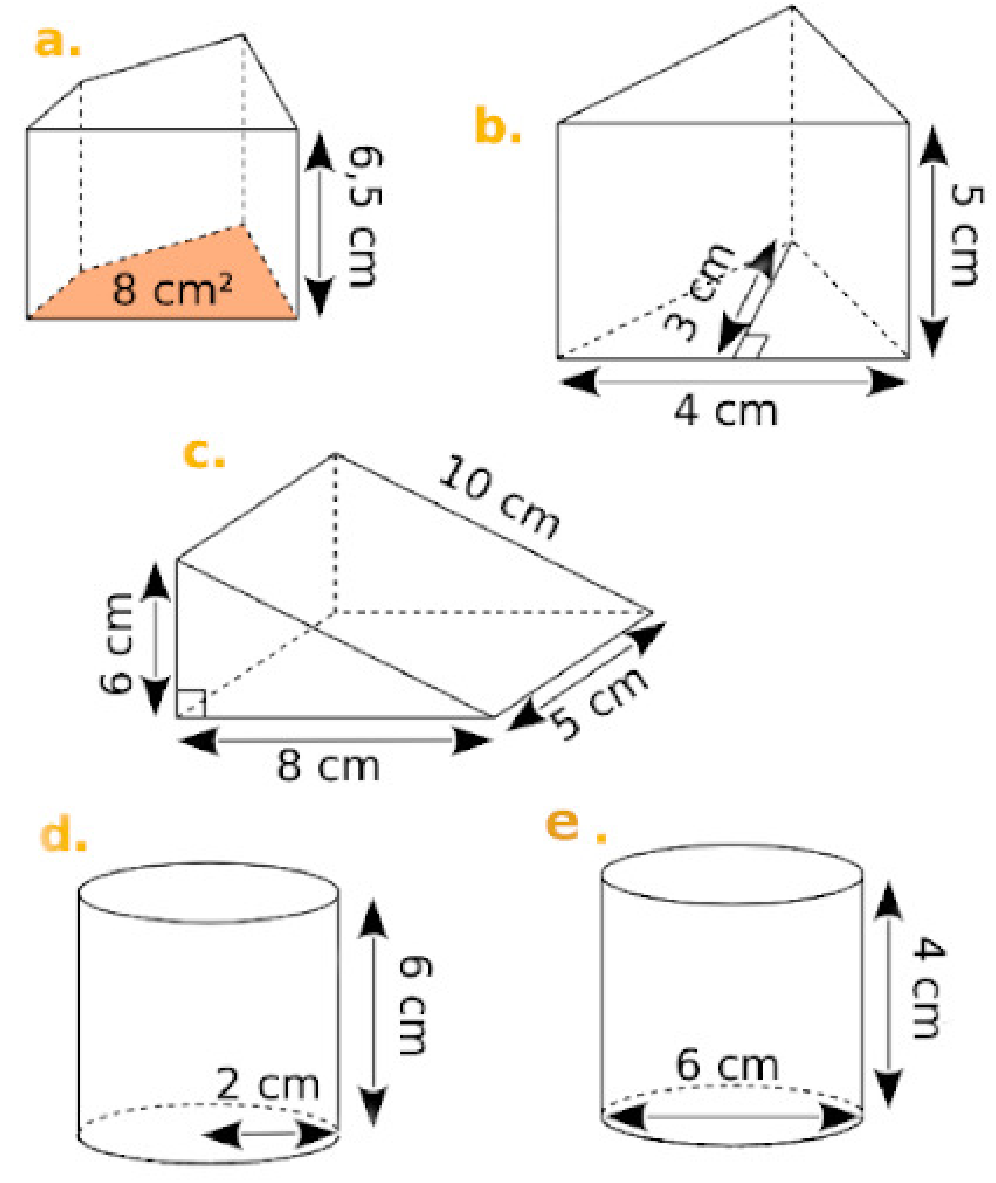
\includegraphics[width=65mm]{prismes_cylindres}
            \end{center}
         \end{exercice}
         
         \begin{Solution}
            \begin{itemize}
               \item[A] $\mathcal{v}_a =\Aire{8}\times\Lg{6,5} =\cor{\Vol[cm]{52}}$ \smallskip
               \item[B] $\mathcal{v}_b =\dfrac{\Lg{4}\times\Lg{3}}{2}\times\Lg{5} =\cor{\Vol[cm]{30}}$ \smallskip
               \item[C] $\mathcal{v}_c =\dfrac{\Lg{8}\times\Lg{6}}{2}\times\Lg{5} =\cor{\Vol[cm]{120}}$ \smallskip
               \item[D] $\mathcal{v}_d =\pi\times(\Lg{2})^2\times\Lg{6} \approx\cor{\Vol[cm]{75,4}}$ \smallskip
               \item[E] $\mathcal{v}_e =\pi\times(\Lg{3})^2\times\Lg{4} \approx\cor{\Vol[cm]{113,1}}$
            \end{itemize}
         \end{Solution}
         
         
         \begin{exercice} %6
            Pour un chantier, un maçon doit construire quatre colonnes en béton de forme cylindrique, de \Lg{50} de rayon et de \Lg[m]{4} de hauteur.
            \begin{enumerate}
               \item Quel est le volume total des colonnes ?
               \item Pour \Vol[m]{1} de béton, il faut \Masse[kg]{400} de ciment, \Capa{460} de sable, \Capa{780} de gravillons et \Capa{200} d'eau. \par
                  Donner la quantité de ciment, de sable, de gravillons et d'eau nécessaire pour les quatre colonnes.
            \end{enumerate}
         \end{exercice}
         
         \begin{Solution}
            \begin{enumerate}
               \item $\mathcal{v} =4\times(\pi\times(\Lg[m]{0,5})^2\times\Lg[m]{4}) \approx \Vol[m]{12,57}$. \par
                  \cor{Le volume des colonnes est d'environ \Vol[m]{12,57}}.
               \item Les valeurs sont pour \Vol[m]{1} donc, il suffit de multiplier toutes les quantités par 12,57 : \par
                  Il faut $12,57\times\Masse[kg]{400} =$ \cor{\Masse[kg]{5028} de ciment} ; \par
                  $12,57\times\Capa{460} \approx$ \cor{\Capa{5 782} de sable} ; \par
                  $12,57\times\Capa{780} \approx$ \cor{\Capa{9 805} de gravillons} ; \par
                  $12,57\times\Capa{200} =$ \cor{\Capa{2 514} d'eau}.
            \end{enumerate}
         \end{Solution}
         
         
         \begin{exercice}[Dur] %7
            Voici la représentation en perspective cavalière d'une maison de poupée dont les longueurs sont exprimées en centimètres.
            \begin{center}
               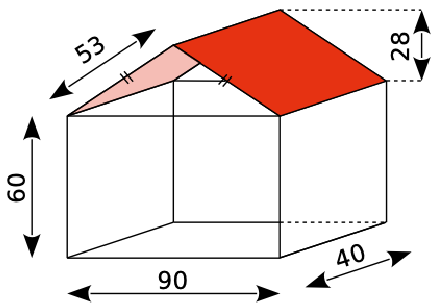
\includegraphics[width=5cm]{maison}
            \end{center}
            \begin{enumerate}
               \item Calculer la surface de bois nécessaire pour réaliser le modèle de la maison.
               \item Sachant que le contre-plaqué choisi coûte \Prix{28,90} le \Aire[m]{}, calculer le montant de sa dépense.
               \item Calculer, au \Vol[dm]{} près, le volume de la maison.
            \end{enumerate}
         \end{exercice}
         
         \begin{Solution}
            \begin{enumerate}
               \item On a les pièces suivantes, les aires sont en \Aire{} :
                  \begin{itemize}
                     \item fond : $90\times40 =3\,600$ ;
                     \item face et arrière : $2\times(90\times60) =\num{10800}$ ;
                     \item côtés : $2\times(40\times60) =\num{4800}$ ; 
                     \item toit : $2\times(40\times53) =\num{4240}$ ; \smallskip
                     \item pignons : $2\times\dfrac{90\times28}{2} =\num{2520}$. \smallskip
                  \end{itemize}
                  On additionne les mesures de toutes les pièces : \par
                  $\num{3600}+\num{10800}+\num{4800}+\num{4240}+\num{2520} =\num{25960}$. \par
                  \cor{Il faut \Aire[m]{2,596} de bois pour la maison}.
               \item $2,596\times28,9 \approx75,02$.  
                  \cor{Le prix est de $\approx\Prix{75}$}.
               \item La maison a la forme d'un prisme de base : \par
                  \Aire{5400} + \Aire{1260} = \Aire{6660} et dont la hauteur vaut \Lg{40}. Son volume est donc de $\Aire{6660}\times\Lg{40} =\Vol[cm]{266400} =\Vol[dm]{266,4}$. \par
                  \cor{Le volume de la maison est d'environ \Vol[dm]{266}}.
            \end{enumerate}
         \end{Solution}

   \end{multicols}

\end{Maquette}


%%% Récré %%%
\begin{Maquette}[Cours]{Theme={Activité récréative},Couleur={IndianRed}}
    
   \ARtitre{Format A5 et cylindres}

      \ARpartie{Chacuneonstruction de cylindres}

         \begin{enumerate}
            \item Découper une feuille au format A4 suivant sa médiane la plus courte afin d'obtenir deux feuilles au format A5.
               \begin{center}
                  \begin{pspicture}(0,0)(3,2.3)
                     \psframe(0,0)(3,2.1)
                     \psline[linestyle=dashed](1.5,0)(1.5,2)
                     \rput(0.75,1){A5}
                     \rput(2.25,1){A5}
                  \end{pspicture}
               \end{center}
            \begin{multicols}{2}
            \item Rouler la première feuille dans le sens de la \par
               longueur pour former un premier cylindre A. \par
               {\psset{unit=0.7}
                  \begin{pspicture}(0.5,-0.5)(11,3.75)
                     \psframe(0,0)(3,2.1)
                     \rput(1.5,1){A5}
                     \rput(4,1){$\Rightarrow$}
                     \psline(5.6,-0.37)(5.6,1.65)
                     \psline(5,0)(5,2)
                     \psline(7,0)(7,2)
                     \psellipticarc(6,2)(1,0.4){0}{-137}
                     \psellipticarc(6,0)(1,0.4){0}{137}
                     \psellipticarc(6,0)(1,0.4){180}{-137}
                     \rput(8,1){$\Rightarrow$}
                     \psline(10.5,0)(10.5,2)
                     \psline(9,0)(9,2)
                     \psellipse(9.75,2)(0.75,0.3)
                     \psellipticarc(9.75,0)(0.75,0.3){180}{0}
                  \end{pspicture}}
            \item Rouler la deuxième feuille dans le sens de la \par
               largeur pour former un deuxième cylindre B. \par
               {\psset{unit=0.71}
                  \begin{pspicture}(0,-0.5)(8.5,3.75)
                     \psframe(0,0)(2.1,3)
                     \rput(1,1.5){A5}
                     \rput(3,1.5){$\Rightarrow$}
                     \psline(4.4,-0.3)(4.4,2.7)
                     \psline(4,0)(4,3)
                     \psline(5.5,0)(5.5,3)
                     \psellipticarc(4.75,3)(0.75,0.35){0}{-137}
                     \psellipticarc(4.75,0)(0.75,0.35){0}{137}
                     \psellipticarc(4.75,0)(0.75,0.35){180}{-137}
                     \rput(6.5,1.5){$\Rightarrow$}
                     \psline(8.5,0)(8.5,3)
                     \psline(7.5,0)(7.5,3)
                     \psellipse(8,3)(0.5,0.25)
                     \psellipticarc(8,0)(0.5,0.25){180}{0}
                  \end{pspicture}}
            \end{multicols}
            \item Selon vous, ces cylindres ont-il le même volume ? Si non, quel est celui qui semble avoir le volume le plus grand ? \pointilles
         \end{enumerate}
         
      \ARpartie{Calcul du volume}
         \begin{enumerate}
         \setcounter{enumi}{4}
            \item Rappeler les dimensions d'une feuille au format A4. En déduire les dimensions d'une feuille au format A5. \par \smallskip
               \pointilles
            \item Premier cylindre.
            \begin{enumerate}
               \item Donner la mesure de la hauteur du cylindre. \pointilles
               \item Que vaut le périmètre du disque de base du cylindre ? En déduire son rayon. \par \smallskip
               \pointilles
               \item Calculer alors  le volume du premier cylindre. \par \smallskip
               \pointilles
            \end{enumerate}
            \item Deuxième cylindre.
            \begin{enumerate}
               \item Donner la mesure de la hauteur du cylindre. \pointilles
               \item Que vaut le périmètre du disque de base du cylindre ? En déduire son rayon. \par \smallskip
               \pointilles
               \item Calculer alors  le volume du deuxième cylindre. \par \smallskip
               \pointilles
            \end{enumerate}
            \item Conclusion : \pointilles \par \medskip
               \pointilles
         \end{enumerate}

\end{Maquette}